
% Default to the notebook output style

    


% Inherit from the specified cell style.




    
\documentclass[11pt]{article}

    
    
    \usepackage[T1]{fontenc}
    % Nicer default font (+ math font) than Computer Modern for most use cases
    \usepackage{mathpazo}

    % Basic figure setup, for now with no caption control since it's done
    % automatically by Pandoc (which extracts ![](path) syntax from Markdown).
    \usepackage{graphicx}
    % We will generate all images so they have a width \maxwidth. This means
    % that they will get their normal width if they fit onto the page, but
    % are scaled down if they would overflow the margins.
    % \makeatletter
    % \def\maxwidth{\ifdim\Gin@nat@width>\linewidth\linewidth
    % \else\Gin@nat@width\fi}
    % \makeatother
    % \let\Oldincludegraphics\includegraphics
    % % Set max figure width to be 80% of text width, for now hardcoded.
    % \renewcommand{\includegraphics}[1]{\Oldincludegraphics[width=.8\maxwidth]{#1}}
    % % Ensure that by default, figures have no caption (until we provide a
    % % proper Figure object with a Caption API and a way to capture that
    % % in the conversion process - todo).
    % \usepackage{caption}
    % \DeclareCaptionLabelFormat{nolabel}{}
    % \captionsetup{labelformat=nolabel}

    \usepackage{adjustbox} % Used to constrain images to a maximum size 
    \usepackage{xcolor} % Allow colors to be defined
    \usepackage{enumerate} % Needed for markdown enumerations to work
    \usepackage{geometry} % Used to adjust the document margins
    \usepackage{amsmath} % Equations
    \usepackage{amssymb} % Equations
    \usepackage{textcomp} % defines textquotesingle
    % Hack from http://tex.stackexchange.com/a/47451/13684:
    \AtBeginDocument{%
        \def\PYZsq{\textquotesingle}% Upright quotes in Pygmentized code
    }
    \usepackage{upquote} % Upright quotes for verbatim code
    \usepackage{eurosym} % defines \euro
    % \usepackage[mathletters]{ucs} % Extended unicode (utf-8) support
    \usepackage[utf8x]{inputenc} % Allow utf-8 characters in the tex document
    \usepackage{fancyvrb} % verbatim replacement that allows latex
    \usepackage{grffile} % extends the file name processing of package graphics 
                         % to support a larger range 
    % The hyperref package gives us a pdf with properly built
    % internal navigation ('pdf bookmarks' for the table of contents,
    % internal cross-reference links, web links for URLs, etc.)
    \usepackage{hyperref}
    \usepackage{longtable} % longtable support required by pandoc >1.10
    \usepackage{booktabs}  % table support for pandoc > 1.12.2
    \usepackage[inline]{enumitem} % IRkernel/repr support (it uses the enumerate* environment)
    \usepackage[normalem]{ulem} % ulem is needed to support strikethroughs (\sout)
                                % normalem makes italics be italics, not underlines
    \usepackage{mathrsfs}
    \usepackage{float}
    \usepackage{biblatex}
    \usepackage[english]{babel}
    \addbibresource{resources.bib}
    
    % \bibliographystyle{annotate}
    % \bibliography{resources.bib}
    
    
    % Colors for the hyperref package
    \definecolor{urlcolor}{rgb}{0,.145,.698}
    \definecolor{linkcolor}{rgb}{.71,0.21,0.01}
    \definecolor{citecolor}{rgb}{.12,.54,.11}

    % ANSI colors
    \definecolor{ansi-black}{HTML}{3E424D}
    \definecolor{ansi-black-intense}{HTML}{282C36}
    \definecolor{ansi-red}{HTML}{E75C58}
    \definecolor{ansi-red-intense}{HTML}{B22B31}
    \definecolor{ansi-green}{HTML}{00A250}
    \definecolor{ansi-green-intense}{HTML}{007427}
    \definecolor{ansi-yellow}{HTML}{DDB62B}
    \definecolor{ansi-yellow-intense}{HTML}{B27D12}
    \definecolor{ansi-blue}{HTML}{208FFB}
    \definecolor{ansi-blue-intense}{HTML}{0065CA}
    \definecolor{ansi-magenta}{HTML}{D160C4}
    \definecolor{ansi-magenta-intense}{HTML}{A03196}
    \definecolor{ansi-cyan}{HTML}{60C6C8}
    \definecolor{ansi-cyan-intense}{HTML}{258F8F}
    \definecolor{ansi-white}{HTML}{C5C1B4}
    \definecolor{ansi-white-intense}{HTML}{A1A6B2}
    \definecolor{ansi-default-inverse-fg}{HTML}{FFFFFF}
    \definecolor{ansi-default-inverse-bg}{HTML}{000000}

    % commands and environments needed by pandoc snippets
    % extracted from the output of `pandoc -s`
    \providecommand{\tightlist}{%
      \setlength{\itemsep}{0pt}\setlength{\parskip}{0pt}}
    \DefineVerbatimEnvironment{Highlighting}{Verbatim}{commandchars=\\\{\}}
    % Add ',fontsize=\small' for more characters per line
    \newenvironment{Shaded}{}{}
    \newcommand{\KeywordTok}[1]{\textcolor[rgb]{0.00,0.44,0.13}{\textbf{{#1}}}}
    \newcommand{\DataTypeTok}[1]{\textcolor[rgb]{0.56,0.13,0.00}{{#1}}}
    \newcommand{\DecValTok}[1]{\textcolor[rgb]{0.25,0.63,0.44}{{#1}}}
    \newcommand{\BaseNTok}[1]{\textcolor[rgb]{0.25,0.63,0.44}{{#1}}}
    \newcommand{\FloatTok}[1]{\textcolor[rgb]{0.25,0.63,0.44}{{#1}}}
    \newcommand{\CharTok}[1]{\textcolor[rgb]{0.25,0.44,0.63}{{#1}}}
    \newcommand{\StringTok}[1]{\textcolor[rgb]{0.25,0.44,0.63}{{#1}}}
    \newcommand{\CommentTok}[1]{\textcolor[rgb]{0.38,0.63,0.69}{\textit{{#1}}}}
    \newcommand{\OtherTok}[1]{\textcolor[rgb]{0.00,0.44,0.13}{{#1}}}
    \newcommand{\AlertTok}[1]{\textcolor[rgb]{1.00,0.00,0.00}{\textbf{{#1}}}}
    \newcommand{\FunctionTok}[1]{\textcolor[rgb]{0.02,0.16,0.49}{{#1}}}
    \newcommand{\RegionMarkerTok}[1]{{#1}}
    \newcommand{\ErrorTok}[1]{\textcolor[rgb]{1.00,0.00,0.00}{\textbf{{#1}}}}
    \newcommand{\NormalTok}[1]{{#1}}
    
    % Additional commands for more recent versions of Pandoc
    \newcommand{\ConstantTok}[1]{\textcolor[rgb]{0.53,0.00,0.00}{{#1}}}
    \newcommand{\SpecialCharTok}[1]{\textcolor[rgb]{0.25,0.44,0.63}{{#1}}}
    \newcommand{\VerbatimStringTok}[1]{\textcolor[rgb]{0.25,0.44,0.63}{{#1}}}
    \newcommand{\SpecialStringTok}[1]{\textcolor[rgb]{0.73,0.40,0.53}{{#1}}}
    \newcommand{\ImportTok}[1]{{#1}}
    \newcommand{\DocumentationTok}[1]{\textcolor[rgb]{0.73,0.13,0.13}{\textit{{#1}}}}
    \newcommand{\AnnotationTok}[1]{\textcolor[rgb]{0.38,0.63,0.69}{\textbf{\textit{{#1}}}}}
    \newcommand{\CommentVarTok}[1]{\textcolor[rgb]{0.38,0.63,0.69}{\textbf{\textit{{#1}}}}}
    \newcommand{\VariableTok}[1]{\textcolor[rgb]{0.10,0.09,0.49}{{#1}}}
    \newcommand{\ControlFlowTok}[1]{\textcolor[rgb]{0.00,0.44,0.13}{\textbf{{#1}}}}
    \newcommand{\OperatorTok}[1]{\textcolor[rgb]{0.40,0.40,0.40}{{#1}}}
    \newcommand{\BuiltInTok}[1]{{#1}}
    \newcommand{\ExtensionTok}[1]{{#1}}
    \newcommand{\PreprocessorTok}[1]{\textcolor[rgb]{0.74,0.48,0.00}{{#1}}}
    \newcommand{\AttributeTok}[1]{\textcolor[rgb]{0.49,0.56,0.16}{{#1}}}
    \newcommand{\InformationTok}[1]{\textcolor[rgb]{0.38,0.63,0.69}{\textbf{\textit{{#1}}}}}
    \newcommand{\WarningTok}[1]{\textcolor[rgb]{0.38,0.63,0.69}{\textbf{\textit{{#1}}}}}
    
    
    % Define a nice break command that doesn't care if a line doesn't already
    % exist.
    \def\br{\hspace*{\fill} \\* }
    % Math Jax compatibility definitions
    \def\gt{>}
    \def\lt{<}
    \let\Oldtex\TeX
    \let\Oldlatex\LaTeX
    \renewcommand{\TeX}{\textrm{\Oldtex}}
    \renewcommand{\LaTeX}{\textrm{\Oldlatex}}
    % Document parameters
    % Document title
    \title{Race and Incarceration in America}
    
    \date{December 12, 2019}
    
    
    

%     % Pygments definitions
    
\makeatletter
\def\PY@reset{\let\PY@it=\relax \let\PY@bf=\relax%
    \let\PY@ul=\relax \let\PY@tc=\relax%
    \let\PY@bc=\relax \let\PY@ff=\relax}
\def\PY@tok#1{\csname PY@tok@#1\endcsname}
\def\PY@toks#1+{\ifx\relax#1\empty\else%
    \PY@tok{#1}\expandafter\PY@toks\fi}
\def\PY@do#1{\PY@bc{\PY@tc{\PY@ul{%
    \PY@it{\PY@bf{\PY@ff{#1}}}}}}}
\def\PY#1#2{\PY@reset\PY@toks#1+\relax+\PY@do{#2}}

\expandafter\def\csname PY@tok@w\endcsname{\def\PY@tc##1{\textcolor[rgb]{0.73,0.73,0.73}{##1}}}
\expandafter\def\csname PY@tok@c\endcsname{\let\PY@it=\textit\def\PY@tc##1{\textcolor[rgb]{0.25,0.50,0.50}{##1}}}
\expandafter\def\csname PY@tok@cp\endcsname{\def\PY@tc##1{\textcolor[rgb]{0.74,0.48,0.00}{##1}}}
\expandafter\def\csname PY@tok@k\endcsname{\let\PY@bf=\textbf\def\PY@tc##1{\textcolor[rgb]{0.00,0.50,0.00}{##1}}}
\expandafter\def\csname PY@tok@kp\endcsname{\def\PY@tc##1{\textcolor[rgb]{0.00,0.50,0.00}{##1}}}
\expandafter\def\csname PY@tok@kt\endcsname{\def\PY@tc##1{\textcolor[rgb]{0.69,0.00,0.25}{##1}}}
\expandafter\def\csname PY@tok@o\endcsname{\def\PY@tc##1{\textcolor[rgb]{0.40,0.40,0.40}{##1}}}
\expandafter\def\csname PY@tok@ow\endcsname{\let\PY@bf=\textbf\def\PY@tc##1{\textcolor[rgb]{0.67,0.13,1.00}{##1}}}
\expandafter\def\csname PY@tok@nb\endcsname{\def\PY@tc##1{\textcolor[rgb]{0.00,0.50,0.00}{##1}}}
\expandafter\def\csname PY@tok@nf\endcsname{\def\PY@tc##1{\textcolor[rgb]{0.00,0.00,1.00}{##1}}}
\expandafter\def\csname PY@tok@nc\endcsname{\let\PY@bf=\textbf\def\PY@tc##1{\textcolor[rgb]{0.00,0.00,1.00}{##1}}}
\expandafter\def\csname PY@tok@nn\endcsname{\let\PY@bf=\textbf\def\PY@tc##1{\textcolor[rgb]{0.00,0.00,1.00}{##1}}}
\expandafter\def\csname PY@tok@ne\endcsname{\let\PY@bf=\textbf\def\PY@tc##1{\textcolor[rgb]{0.82,0.25,0.23}{##1}}}
\expandafter\def\csname PY@tok@nv\endcsname{\def\PY@tc##1{\textcolor[rgb]{0.10,0.09,0.49}{##1}}}
\expandafter\def\csname PY@tok@no\endcsname{\def\PY@tc##1{\textcolor[rgb]{0.53,0.00,0.00}{##1}}}
\expandafter\def\csname PY@tok@nl\endcsname{\def\PY@tc##1{\textcolor[rgb]{0.63,0.63,0.00}{##1}}}
\expandafter\def\csname PY@tok@ni\endcsname{\let\PY@bf=\textbf\def\PY@tc##1{\textcolor[rgb]{0.60,0.60,0.60}{##1}}}
\expandafter\def\csname PY@tok@na\endcsname{\def\PY@tc##1{\textcolor[rgb]{0.49,0.56,0.16}{##1}}}
\expandafter\def\csname PY@tok@nt\endcsname{\let\PY@bf=\textbf\def\PY@tc##1{\textcolor[rgb]{0.00,0.50,0.00}{##1}}}
\expandafter\def\csname PY@tok@nd\endcsname{\def\PY@tc##1{\textcolor[rgb]{0.67,0.13,1.00}{##1}}}
\expandafter\def\csname PY@tok@s\endcsname{\def\PY@tc##1{\textcolor[rgb]{0.73,0.13,0.13}{##1}}}
\expandafter\def\csname PY@tok@sd\endcsname{\let\PY@it=\textit\def\PY@tc##1{\textcolor[rgb]{0.73,0.13,0.13}{##1}}}
\expandafter\def\csname PY@tok@si\endcsname{\let\PY@bf=\textbf\def\PY@tc##1{\textcolor[rgb]{0.73,0.40,0.53}{##1}}}
\expandafter\def\csname PY@tok@se\endcsname{\let\PY@bf=\textbf\def\PY@tc##1{\textcolor[rgb]{0.73,0.40,0.13}{##1}}}
\expandafter\def\csname PY@tok@sr\endcsname{\def\PY@tc##1{\textcolor[rgb]{0.73,0.40,0.53}{##1}}}
\expandafter\def\csname PY@tok@ss\endcsname{\def\PY@tc##1{\textcolor[rgb]{0.10,0.09,0.49}{##1}}}
\expandafter\def\csname PY@tok@sx\endcsname{\def\PY@tc##1{\textcolor[rgb]{0.00,0.50,0.00}{##1}}}
\expandafter\def\csname PY@tok@m\endcsname{\def\PY@tc##1{\textcolor[rgb]{0.40,0.40,0.40}{##1}}}
\expandafter\def\csname PY@tok@gh\endcsname{\let\PY@bf=\textbf\def\PY@tc##1{\textcolor[rgb]{0.00,0.00,0.50}{##1}}}
\expandafter\def\csname PY@tok@gu\endcsname{\let\PY@bf=\textbf\def\PY@tc##1{\textcolor[rgb]{0.50,0.00,0.50}{##1}}}
\expandafter\def\csname PY@tok@gd\endcsname{\def\PY@tc##1{\textcolor[rgb]{0.63,0.00,0.00}{##1}}}
\expandafter\def\csname PY@tok@gi\endcsname{\def\PY@tc##1{\textcolor[rgb]{0.00,0.63,0.00}{##1}}}
\expandafter\def\csname PY@tok@gr\endcsname{\def\PY@tc##1{\textcolor[rgb]{1.00,0.00,0.00}{##1}}}
\expandafter\def\csname PY@tok@ge\endcsname{\let\PY@it=\textit}
\expandafter\def\csname PY@tok@gs\endcsname{\let\PY@bf=\textbf}
\expandafter\def\csname PY@tok@gp\endcsname{\let\PY@bf=\textbf\def\PY@tc##1{\textcolor[rgb]{0.00,0.00,0.50}{##1}}}
\expandafter\def\csname PY@tok@go\endcsname{\def\PY@tc##1{\textcolor[rgb]{0.53,0.53,0.53}{##1}}}
\expandafter\def\csname PY@tok@gt\endcsname{\def\PY@tc##1{\textcolor[rgb]{0.00,0.27,0.87}{##1}}}
\expandafter\def\csname PY@tok@err\endcsname{\def\PY@bc##1{\setlength{\fboxsep}{0pt}\fcolorbox[rgb]{1.00,0.00,0.00}{1,1,1}{\strut ##1}}}
\expandafter\def\csname PY@tok@kc\endcsname{\let\PY@bf=\textbf\def\PY@tc##1{\textcolor[rgb]{0.00,0.50,0.00}{##1}}}
\expandafter\def\csname PY@tok@kd\endcsname{\let\PY@bf=\textbf\def\PY@tc##1{\textcolor[rgb]{0.00,0.50,0.00}{##1}}}
\expandafter\def\csname PY@tok@kn\endcsname{\let\PY@bf=\textbf\def\PY@tc##1{\textcolor[rgb]{0.00,0.50,0.00}{##1}}}
\expandafter\def\csname PY@tok@kr\endcsname{\let\PY@bf=\textbf\def\PY@tc##1{\textcolor[rgb]{0.00,0.50,0.00}{##1}}}
\expandafter\def\csname PY@tok@bp\endcsname{\def\PY@tc##1{\textcolor[rgb]{0.00,0.50,0.00}{##1}}}
\expandafter\def\csname PY@tok@fm\endcsname{\def\PY@tc##1{\textcolor[rgb]{0.00,0.00,1.00}{##1}}}
\expandafter\def\csname PY@tok@vc\endcsname{\def\PY@tc##1{\textcolor[rgb]{0.10,0.09,0.49}{##1}}}
\expandafter\def\csname PY@tok@vg\endcsname{\def\PY@tc##1{\textcolor[rgb]{0.10,0.09,0.49}{##1}}}
\expandafter\def\csname PY@tok@vi\endcsname{\def\PY@tc##1{\textcolor[rgb]{0.10,0.09,0.49}{##1}}}
\expandafter\def\csname PY@tok@vm\endcsname{\def\PY@tc##1{\textcolor[rgb]{0.10,0.09,0.49}{##1}}}
\expandafter\def\csname PY@tok@sa\endcsname{\def\PY@tc##1{\textcolor[rgb]{0.73,0.13,0.13}{##1}}}
\expandafter\def\csname PY@tok@sb\endcsname{\def\PY@tc##1{\textcolor[rgb]{0.73,0.13,0.13}{##1}}}
\expandafter\def\csname PY@tok@sc\endcsname{\def\PY@tc##1{\textcolor[rgb]{0.73,0.13,0.13}{##1}}}
\expandafter\def\csname PY@tok@dl\endcsname{\def\PY@tc##1{\textcolor[rgb]{0.73,0.13,0.13}{##1}}}
\expandafter\def\csname PY@tok@s2\endcsname{\def\PY@tc##1{\textcolor[rgb]{0.73,0.13,0.13}{##1}}}
\expandafter\def\csname PY@tok@sh\endcsname{\def\PY@tc##1{\textcolor[rgb]{0.73,0.13,0.13}{##1}}}
\expandafter\def\csname PY@tok@s1\endcsname{\def\PY@tc##1{\textcolor[rgb]{0.73,0.13,0.13}{##1}}}
\expandafter\def\csname PY@tok@mb\endcsname{\def\PY@tc##1{\textcolor[rgb]{0.40,0.40,0.40}{##1}}}
\expandafter\def\csname PY@tok@mf\endcsname{\def\PY@tc##1{\textcolor[rgb]{0.40,0.40,0.40}{##1}}}
\expandafter\def\csname PY@tok@mh\endcsname{\def\PY@tc##1{\textcolor[rgb]{0.40,0.40,0.40}{##1}}}
\expandafter\def\csname PY@tok@mi\endcsname{\def\PY@tc##1{\textcolor[rgb]{0.40,0.40,0.40}{##1}}}
\expandafter\def\csname PY@tok@il\endcsname{\def\PY@tc##1{\textcolor[rgb]{0.40,0.40,0.40}{##1}}}
\expandafter\def\csname PY@tok@mo\endcsname{\def\PY@tc##1{\textcolor[rgb]{0.40,0.40,0.40}{##1}}}
\expandafter\def\csname PY@tok@ch\endcsname{\let\PY@it=\textit\def\PY@tc##1{\textcolor[rgb]{0.25,0.50,0.50}{##1}}}
\expandafter\def\csname PY@tok@cm\endcsname{\let\PY@it=\textit\def\PY@tc##1{\textcolor[rgb]{0.25,0.50,0.50}{##1}}}
\expandafter\def\csname PY@tok@cpf\endcsname{\let\PY@it=\textit\def\PY@tc##1{\textcolor[rgb]{0.25,0.50,0.50}{##1}}}
\expandafter\def\csname PY@tok@c1\endcsname{\let\PY@it=\textit\def\PY@tc##1{\textcolor[rgb]{0.25,0.50,0.50}{##1}}}
\expandafter\def\csname PY@tok@cs\endcsname{\let\PY@it=\textit\def\PY@tc##1{\textcolor[rgb]{0.25,0.50,0.50}{##1}}}

\def\PYZbs{\char`\\}
\def\PYZus{\char`\_}
\def\PYZob{\char`\{}
\def\PYZcb{\char`\}}
\def\PYZca{\char`\^}
\def\PYZam{\char`\&}
\def\PYZlt{\char`\<}
\def\PYZgt{\char`\>}
\def\PYZsh{\char`\#}
\def\PYZpc{\char`\%}
\def\PYZdl{\char`\$}
\def\PYZhy{\char`\-}
\def\PYZsq{\char`\'}
\def\PYZdq{\char`\"}
\def\PYZti{\char`\~}
% for compatibility with earlier versions
\def\PYZat{@}
\def\PYZlb{[}
\def\PYZrb{]}
\makeatother


%     % Exact colors from NB
    \definecolor{incolor}{rgb}{0.0, 0.0, 0.5}
    \definecolor{outcolor}{rgb}{0.545, 0.0, 0.0}



    
    % Prevent overflowing lines due to hard-to-break entities
    \sloppy 
    % Setup hyperref package
    \hypersetup{
      breaklinks=true,  % so long urls are correctly broken across lines
      colorlinks=true,
      urlcolor=urlcolor,
      linkcolor=linkcolor,
      citecolor=citecolor,
      }
    % Slightly bigger margins than the latex defaults
    
    \geometry{verbose,tmargin=1in,bmargin=1in,lmargin=1in,rmargin=1in}
    
    

    \begin{document}
    
    
    \maketitle
    
    

    

    
    \hypertarget{introduction}{%
\section{Introduction}\label{introduction}}

The United States' criminal justice system is a large complicated
machine that seeks to deliver justice when an offense has been
committed. This system has been slowly evolving as our society and
culture have been changing. Many things that Americans take as natural
in our criminal justice systems are quite abnormal among justice systems
worldwide. Since the 1990s, America has seen a drastic increase in the
incarcerated population, despite a sharp decrease in crime\cite{nyt1}.
Many Americans may believe that this drastic increase in incarceration
is a result of increased rates of crime, and that this heightened rate
is natural and just. To many, it is unclear who is most affected by this
drastic change in the application of justice in America, and even more
unclear is how they are so affected.

There is a lot of existing research exploring incarceration and the
criminal justice system. There is a consensus that America incarcerates
a larger proportion of its population than any other nation and that
people of color are disproportionately affected by this high
incarceration rate\cite{nyt2}.

In this project I am interested in exploring the ways in which the law
is being applied differently to people in America. I will explore
different ways to quantify claims about mass incarceration and racial
bias. I will also be examining things that factor into sentence length
including the offense committed and race. There are many things that
contribute to sentence length, however the scope of this project is
limited to these factors.

    \hypertarget{data}{%
\section{Data}\label{data}}

\hypertarget{source-and-credibility}{%
\subsection{Source and Credibility}\label{source-and-credibility}}

The data that I will be using in this analysis is gathered from
primarily two sources. The first is the Bureau of Justice Statistics and
the second is a link to a
\href{https://catalog.data.gov/dataset/sentenced-inmates-in-correctional-facilities}{database}
hosted on \href{https://www.data.gov}{Data.gov} and maintained by the
State of Connecticut Department of Corrections. These are highly
credible sources because they are primary sources for the data. These
organizations are official government agencies which collect, maintain,
and report on this data.

\hypertarget{gathering-and-cleaning}{%
\subsection{Gathering and Cleaning}\label{gathering-and-cleaning}}

All the data which I am using in this report are freely available to the
public. Collection and cleaning was relatively simple as the source data
was well maintained. The data that I collected from the Bureau of
Justice Statistics (BJS) needed to be formatted in a way that is easily
read by the Python packages I will be using. This data was prepared in
.xlsx files as to be easily human readable, however this is not
generally easily ingested by programs. I extracted data that I found to
be relevant into separate .csv files and kept the original files for
reference. The files are

\begin{verbatim}
incarceration_counts.csv
incarceration_by_race.csv
crime_data.csv.
\end{verbatim}

The file that I obtained from the Connecticut Department of Corrections
is a very well maintained database. The largest issue I had with this
file was mild inconsistency with the way in which certain data was
encoded (ex. race was encoded as both \texttt{WHITE} and
\texttt{WHITE\textbackslash{}t}). This was the data that I spent the
most time working to engineer as it is a data set that I intend to use
for different regression-related analyses. The files are

\begin{verbatim}
individuals.csv
regression_df.csv.
\end{verbatim}

    \hypertarget{contents}{%
\subsection{Contents}\label{contents}}

\hypertarget{bureau-of-justice-statistics-data}{%
\subsubsection{Bureau of Justice Statistics
Data}\label{bureau-of-justice-statistics-data}}

Here I will describe generally each data file and its contents, as well
as give a small sample from each file {[}3,4,5{]}.

    First we will examine \texttt{incarceration\_trends.csv}. This data set
records total jail and prison populations across the United States over
time. This is useful in understanding general trends in the U.S. over
time. The prison population columns are raw populations of incarcerated
individuals while the ``population'' column is the U.S. population in
millions for that year.

    \begin{Verbatim}[commandchars=\\\{\}]
    Year  State prisons  Population
24  1949         146881      149.19
61  1986         485553      240.13
75  2000        1209130      282.16

    \end{Verbatim}

    \texttt{incarceration\_by\_race.csv} contains race demographic data for
incarcerated populations by institution. This will allow us to
understand state incarcerated populations.

    \begin{Verbatim}[commandchars=\\\{\}]
       Geography  Total  White  Black  White\_rate  Black\_rate
42  South Dakota   6327   3708    476         530        4663
3        Arizona  67767  36160   8246         775        3184

    \end{Verbatim}

    \texttt{crime\_data.csv} records crime rates over time in this U.S. This
data set will help us understand how crime relates to incarceration. The
rates are given in offense per 100,000.

    \begin{Verbatim}[commandchars=\\\{\}]
    Year  Violent crime  Murder  Rape  Robbery  Assault
46  2006          473.6     5.8  31.6    150.0    292.0
37  1997          611.0     6.8  35.9    186.2    382.1
9   1969          328.7     7.3  18.5    148.4    154.5

    \end{Verbatim}

    \hypertarget{connecticut-department-of-corrections-data}{%
\subsubsection{Connecticut Department of Corrections
Data}\label{connecticut-department-of-corrections-data}}

    This data set contains individual information for 7.77 million people
that have been processed by the justice system and recorded by the
Connecticut Department of Corrections. Each individual is recorded along
with their age, gender, race, offense, and sentence length, among other
things {[}6{]}.

I also created one-hot encoded versions of this data set in order to run
regressions on the data. Because of the size of the data, the regression
data sets are only random subsets of the larger data set.

Because there is so much to consider in what is found in the data set, I
chose not to engineer more features as to avoid unneeded complexity.

    \begin{Verbatim}[commandchars=\\\{\}]
        LATEST ADMISSION DATE  AGE   RACE  SENTENCE DAYS
4149965            06/22/2018   29  WHITE            731
7570861            01/31/2019   34  WHITE            548
3340323            02/02/2018   43  WHITE            548

    \end{Verbatim}

    We ought to disclose the sample sizes among different races that are
found in the Connecticut Department of Justice data. The sample size for
American Indians and Asians is much smaller than that of Whites,
Hispanics, and Blacks, hence we may see some irregular outcomes in the
analysis related to these racial groups.

    \begin{Verbatim}[commandchars=\\\{\}]
Sample size for Blacks: 3287596
Sample size for Whites: 2393949
Sample size for Hispanic: 2039297
Sample size for American Indian: 21133
Sample size for Asian: 35660

    \end{Verbatim}

    \hypertarget{analysis-and-visualization}{%
\section{Analysis and Visualization}\label{analysis-and-visualization}}

\hypertarget{increased-rates}{%
\subsection{Increased Rates}\label{increased-rates}}

Here we can see the drastic increase of the amount of incarceration in
the U.S. Something that is interesting to note is that jails are defined
as places for people who have a sentence less than 1 year, or who are
awaiting trial. So we see that at its peak in 2008, there were more
people awaiting trial than there were being held in federal prison in
1991.

Here I have incarceration rates plotted against the violent crime rate
in the United States. Near the beginning of the crime rate data we might
assume some amount of inaccuracy, since the crime rate seems to be less
than the incarceration rate, however there is an indisputable spike in
crime rates in the 1980s and 1990s. Something to note is that the
incarceration rate seems to lag behind about 20 years. Another thing to
note is that there has been a strict decrease in violent crime (and in
all crime) since the 90s, however we do not see the same decrease in the
incarceration rate.

Some would argue that we see this decrease in crime because of the
increase of incarceration. I would disagree. Consider the scales of the
different curves we see on the chart. Both are in terms of the rate per
100,000, but the crime rate is more than 200 times higher than the
incarceration rate in state prisons. Unless 0.5\% of people who
committed crime in the 90s were committing more than half of all crime,
I would argue that there is some other cause for the decrease in crime
rates.

\begin{figure}[H]
    \centering
    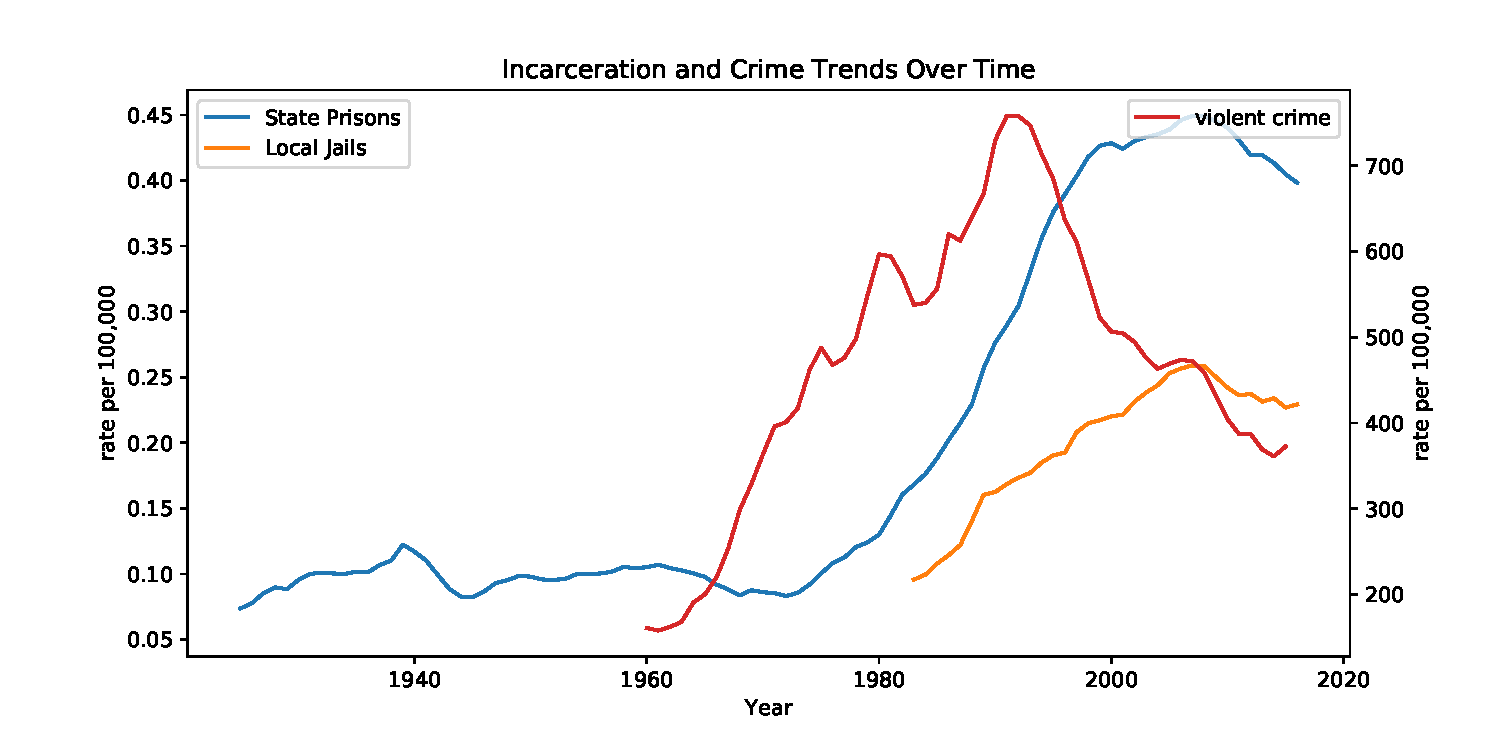
\includegraphics[width=\textwidth]{images/incar_trends.pdf}
    \caption{Incarceration rates over time}
    \label{fig:my_label}
\end{figure}
    
    \hypertarget{artifacts-of-prison-policy}{%
\subsection{Artifacts of Prison
Policy}\label{artifacts-of-prison-policy}}

One might expect sentence lengths to be distributed somewhat smoothly.
However there are standard sentence lengths and mandatory minimum
sentences that influence the distribution of sentence lenghts, making
the distribution not smooth.

\begin{figure}[H]
    \centering
    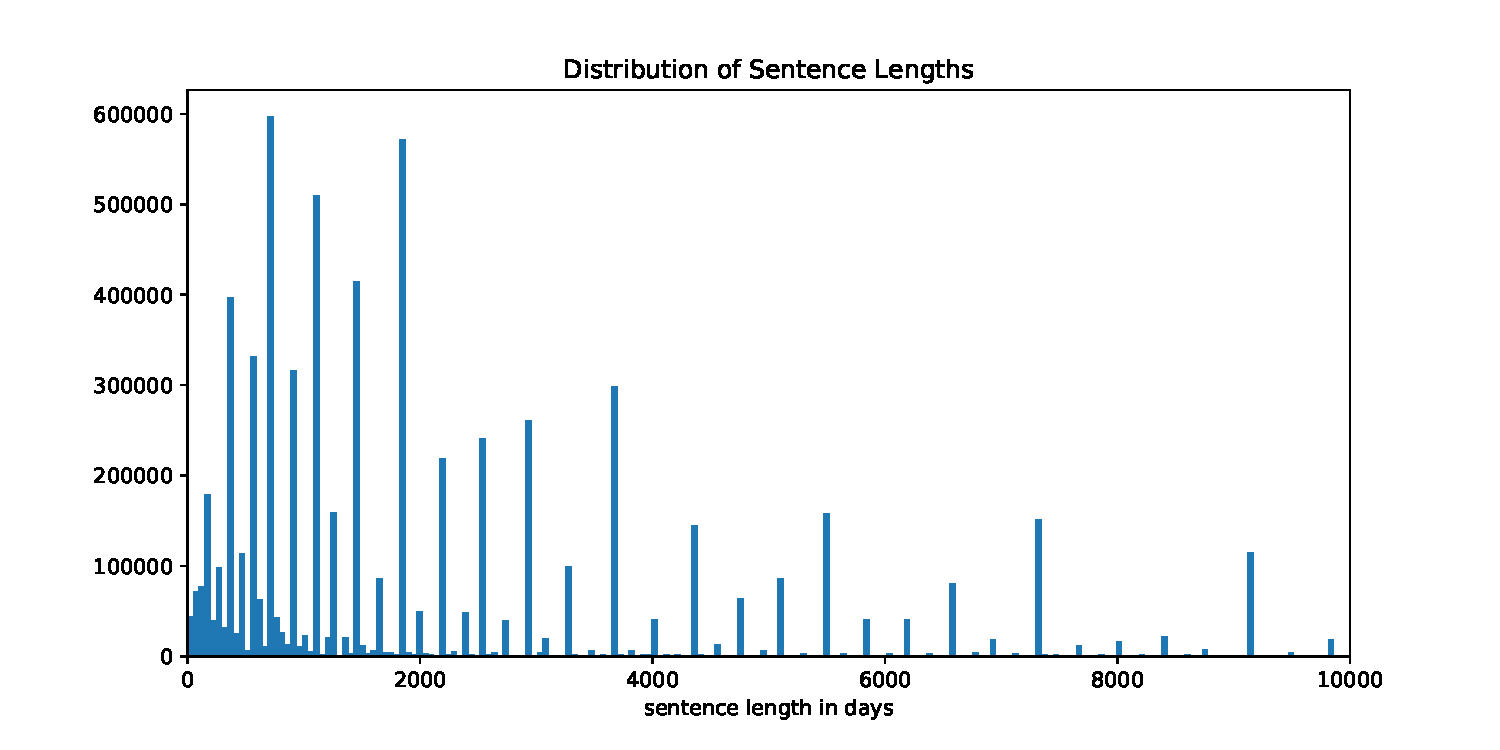
\includegraphics[width=\textwidth]{images/sent_dist.pdf}
    \caption{Distribution of sentences across all inmates in inmates.csv}
    \label{fig:my_label}
\end{figure}
    
    \hypertarget{racial-disparities}{%
\subsection{Racial Disparities}\label{racial-disparities}}

In this section we will explore how the criminal justice system affects
people of different races.

\hypertarget{incarceration-disparity}{%
\subsubsection{Incarceration Disparity}\label{incarceration-disparity}}

These simple histograms, which plot the incarceration rates of Whites,
Blacks, Hispanics, and Asians among the 50 states, show the huge racial
disparity in incarceration in America. By incarceration rate we mean: of
100,000 people of a given race, how many are incarcerated? A simple
examination of the x-axis, which is rate of incarceration shows that the
histogram for Whites barely overlaps with the histograms for Blacks and
Hispanics. This means that in states with a low incarceration rate for
Blacks, the Black incarceration rate is higher than the highest rates
seen among Whites.

\begin{figure}[H]
    \centering
    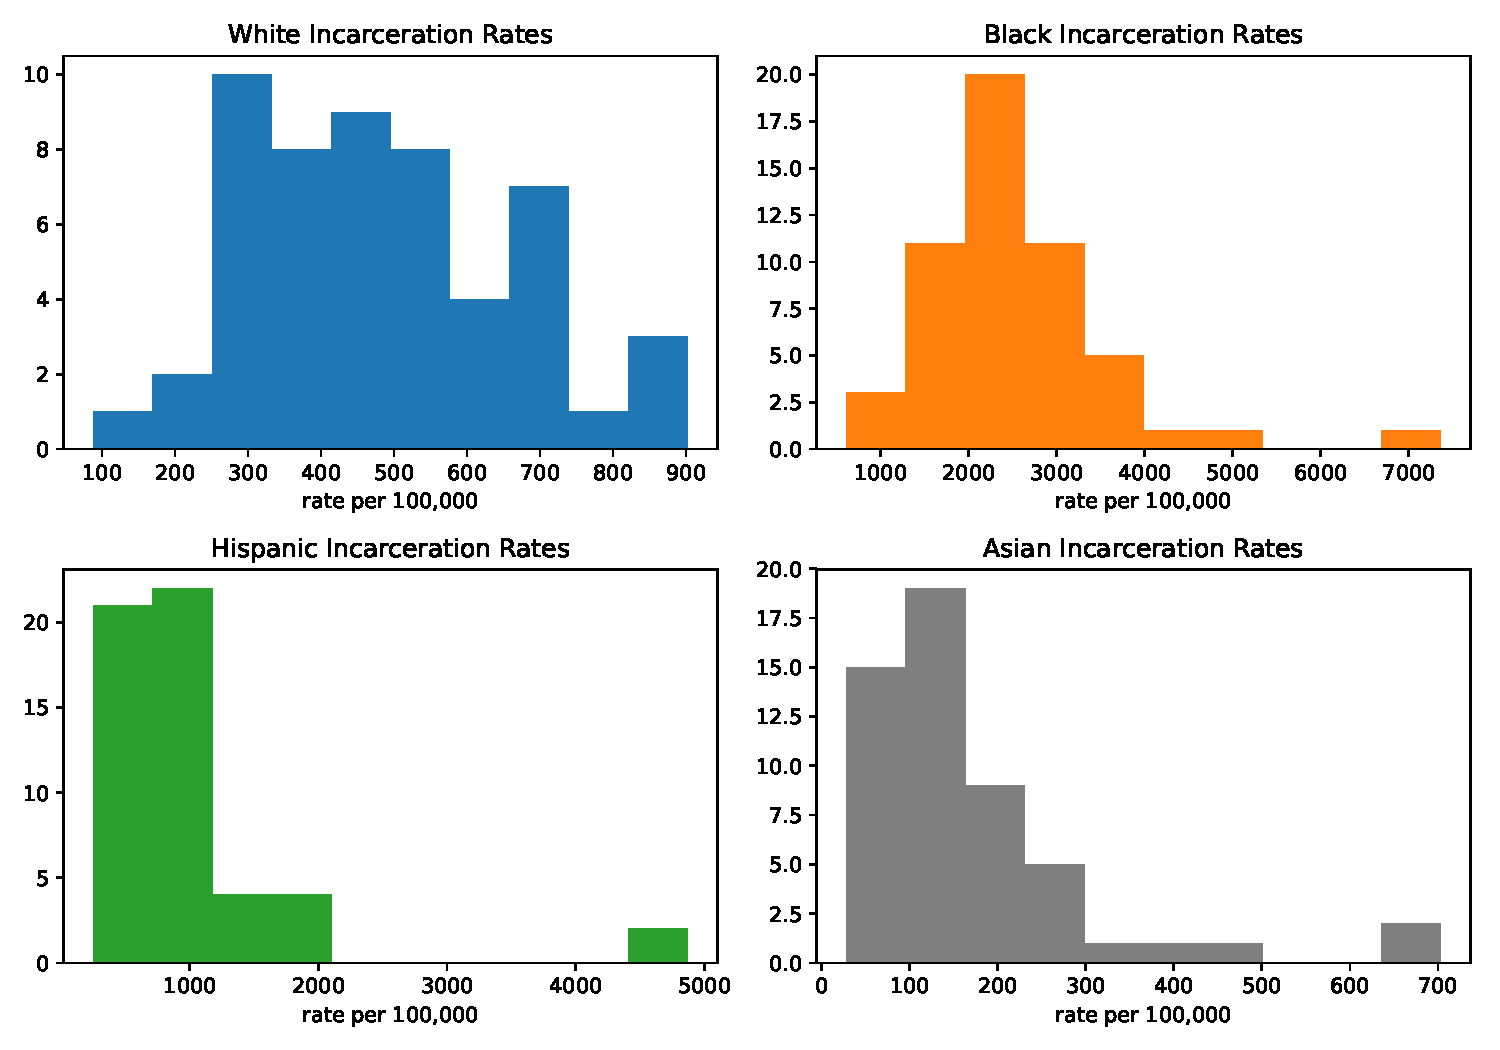
\includegraphics[width=\textwidth]{images/state_incar_rates.pdf}
    \caption{Distribution of states' mean incarceration rate, blocked by race}
    \label{fig:my_label}
\end{figure}
    
    \hypertarget{distribution-of-sentence-lengths}{%
\subsubsection{Distribution of Sentence
Lengths}\label{distribution-of-sentence-lengths}}

The next aspect we will explore in this section is the distribution of
sentence lengths among people of different races. Here we are using the
data of more than 7.7 million individuals processed by the criminal
justice system. The medians are comparable on the scale at which
sentence length is given. Asians and American Indians have the longest
median sentence length, however the standard deviation in their sentence
lengths is much less than what is seen in the other racial groups. I
would attribute this to the low sample size of Asians and American
Indians.

    \begin{Verbatim}[commandchars=\\\{\}]
Median sentence lengths:
 RACE
AMER IND    2192
ASIAN       2557
BLACK       1826
HISPANIC    1826
WHITE       1461
Name: SENTENCE DAYS, dtype: int64


Standard deviation of sentence lengths:
 RACE
AMER IND     3208.584729
ASIAN        5122.011265
BLACK       37306.146883
HISPANIC    35763.282330
WHITE       46882.705552
Name: SENTENCE DAYS, dtype: float64

    \end{Verbatim}

    This box plot is where we begin to see the disparity in the way people
of different races are sentenced. While the first two quartiles of each
racial group's sentence lengths are similar, we see that the top two
quartiles vary widely.

\begin{figure}[H]
    \centering
    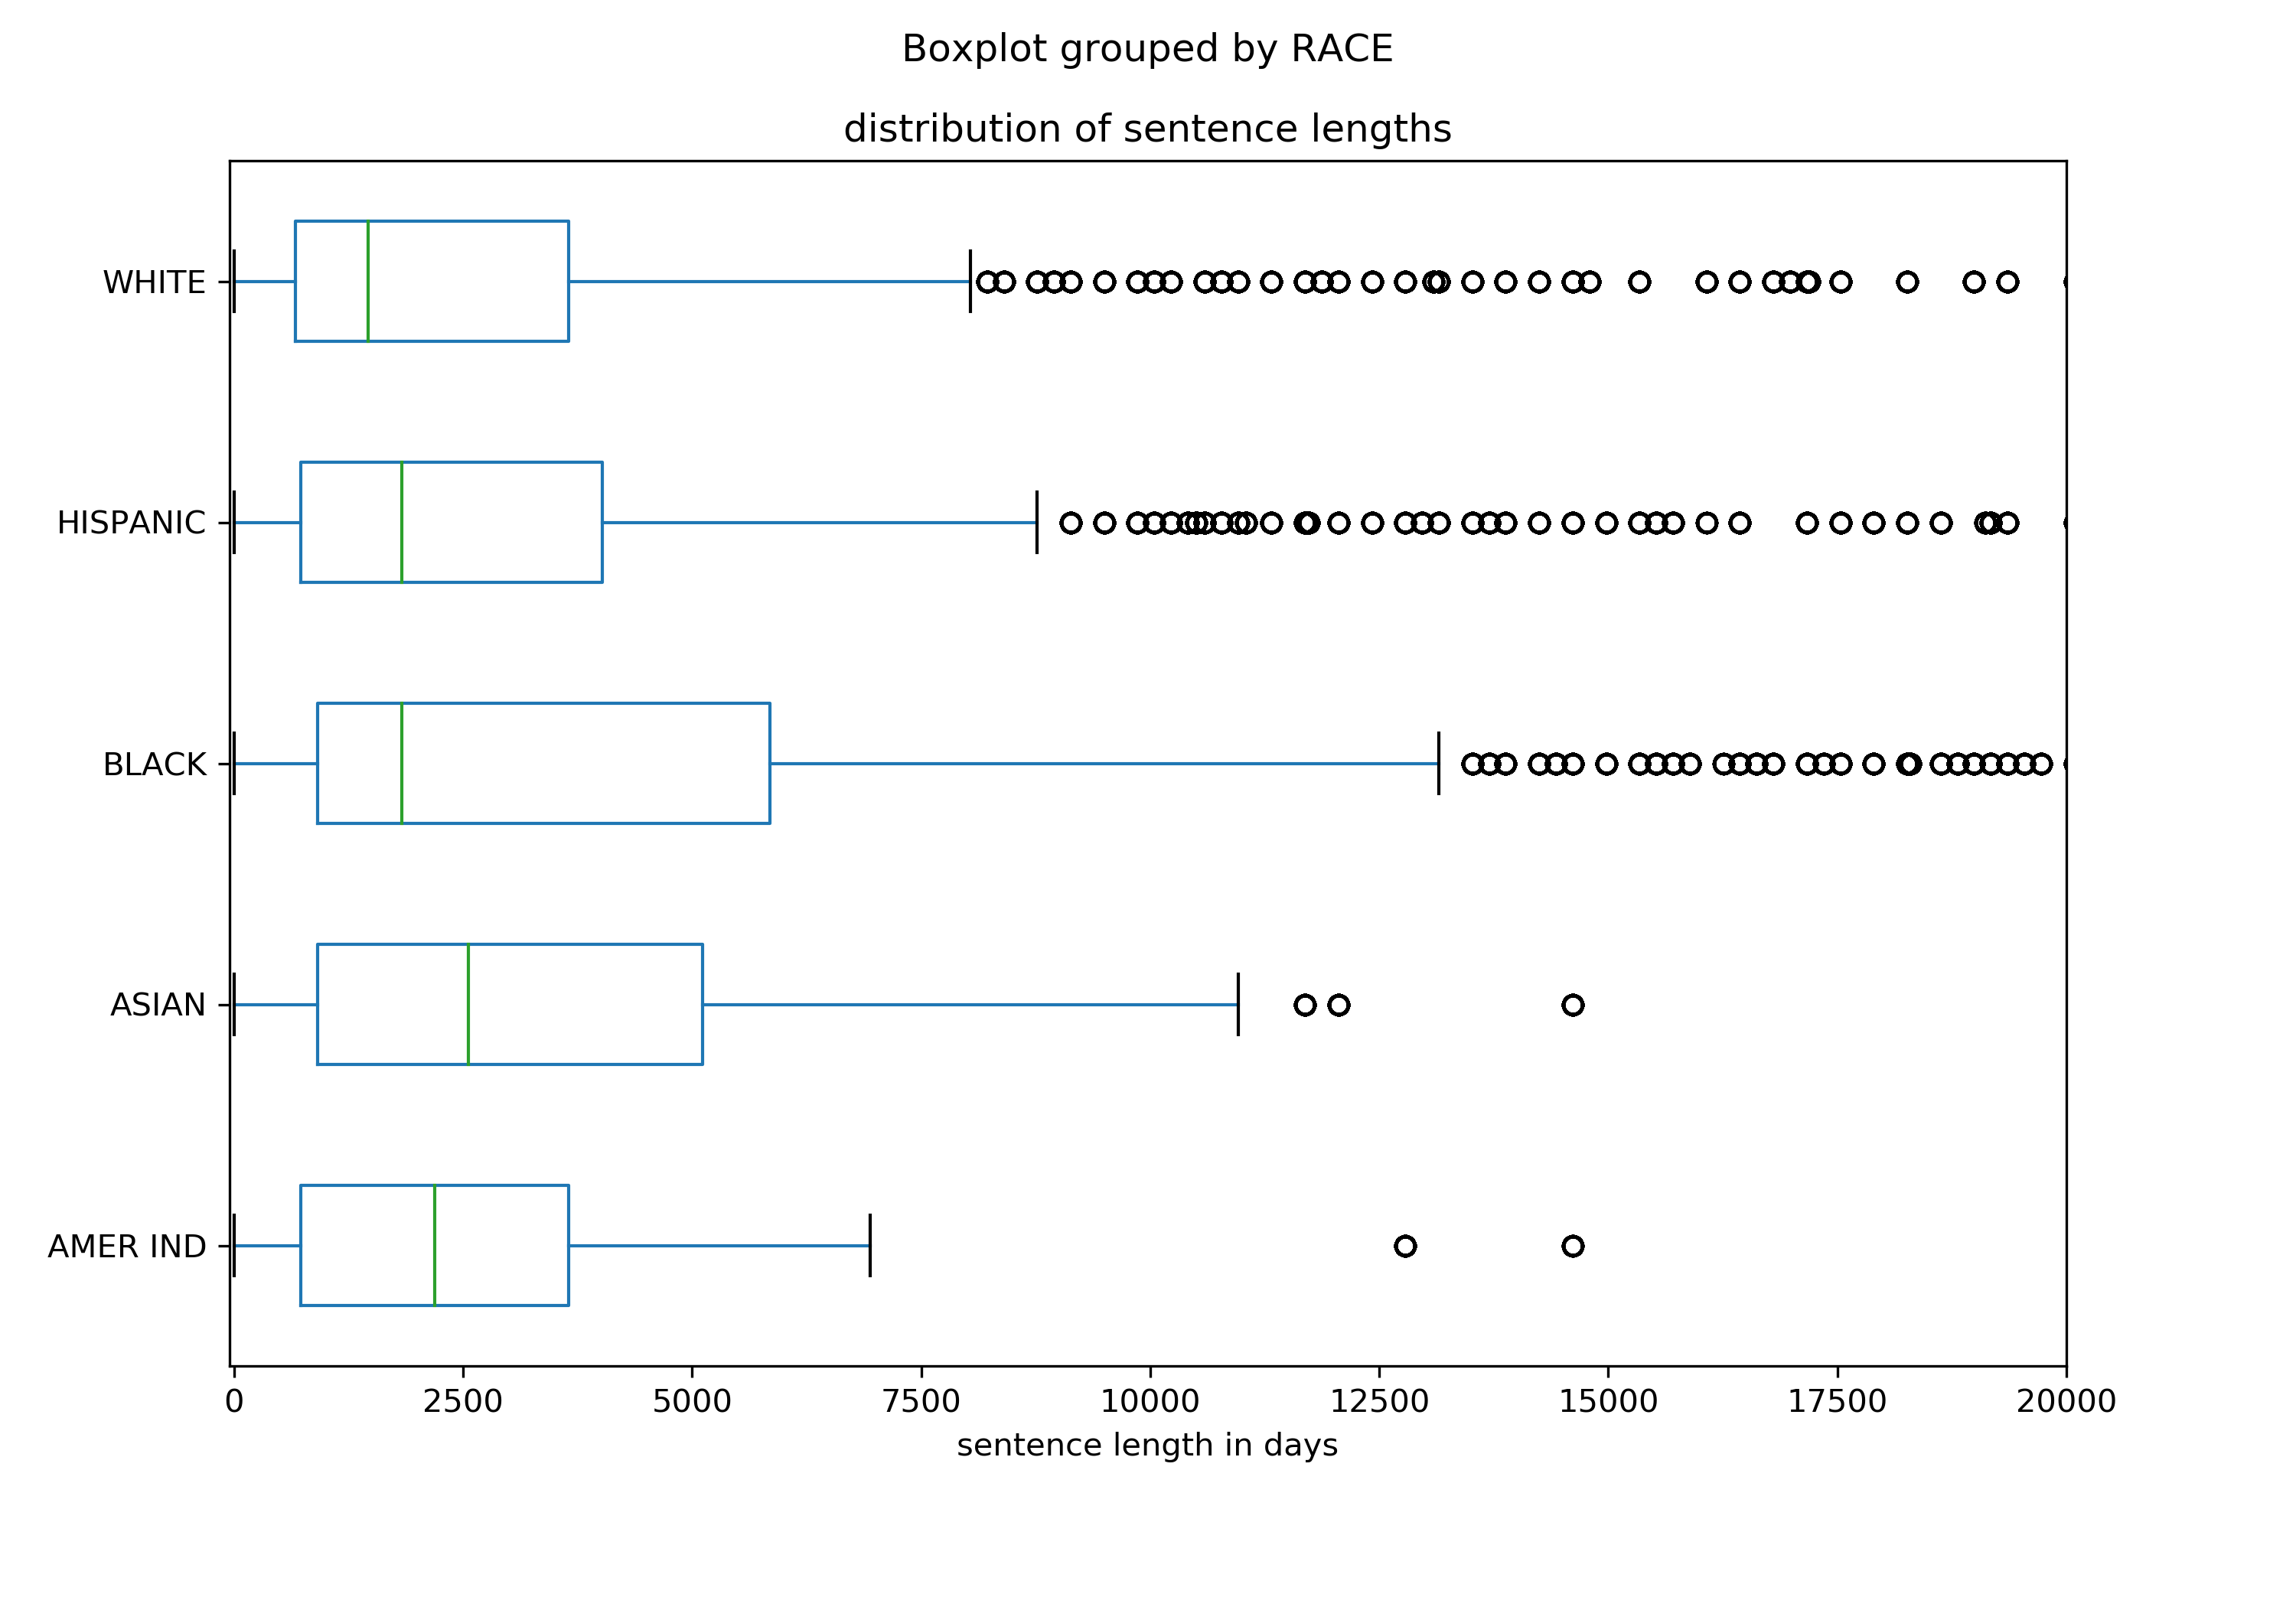
\includegraphics[scale=.6]{images/sentence_boxplot.png}
    \caption{Boxplot distribution of sentence length for inmates in individuals.csv, blocked by race}
    \label{fig:my_label}
\end{figure}
    
    The following histograms will assist us in understanding these
distributions.

\begin{figure}[H]
    \centering
    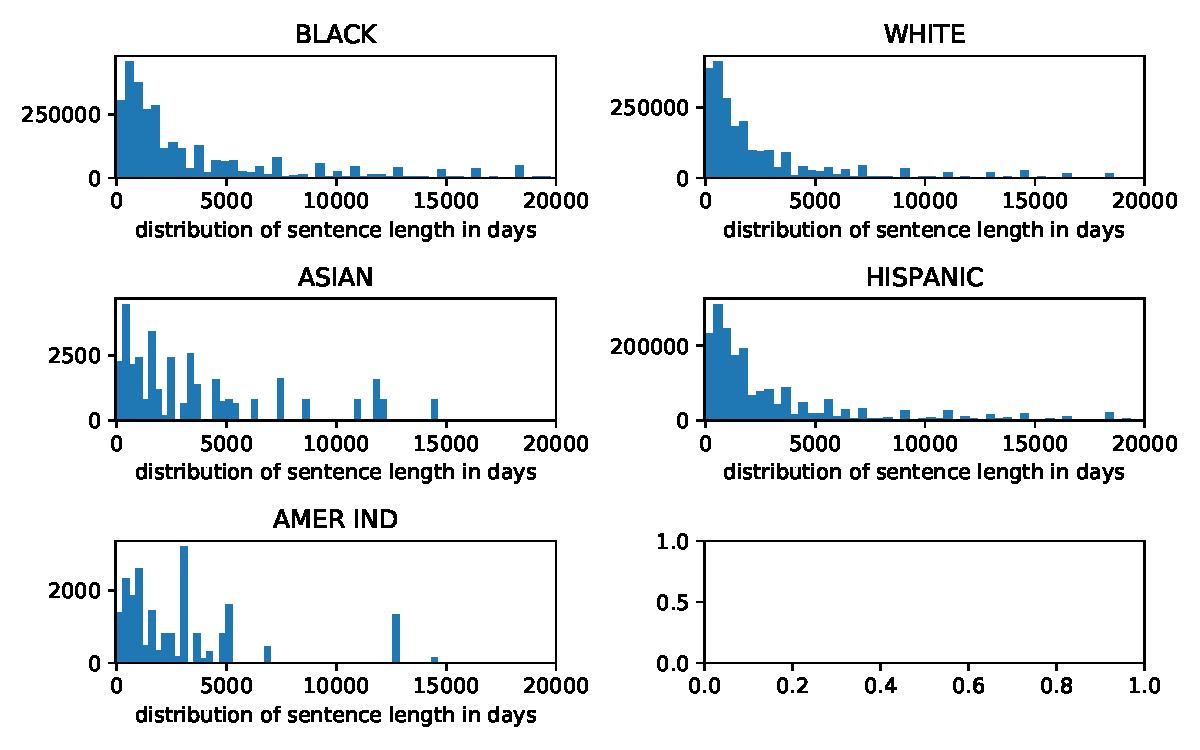
\includegraphics[width=\textwidth]{images/race_sentence_dist.pdf}
    \caption{Histogram distribution of sentence length for inmates in individuals.csv, blocked by race}
    \label{fig:my_label}
\end{figure}
    
    While it may appear that these sentences are distributed fairly
equivalently, we can examine the kurtosis of the distribution to
understand how much of the weight of the distribution is found in the
extremities. Groups with high kurtosis have a higher probability of
receiving a sentence that is far from the mean\cite{kurt}.

As we can see, Blacks and Hispanics have the greatest kurtosis, meaning
they are much more likely to receive an extreme sentence length. It is
difficult to explain the small kurtosis in American Indians and Asians
because of the small sample size.

    \begin{Verbatim}[commandchars=\\\{\}]
White Kurtosis: 54.01344161453346
Black Kurtosis: 86.11479232153843
Hispanic Kurtosis: 96.03075354970996
American Indian Kurtosis: 4.0085627062942955
Asian Kurtosis: 7.45297417968173

    \end{Verbatim}

    \hypertarget{predicting-sentence-length}{%
\subsubsection{Predicting Sentence
Length}\label{predicting-sentence-length}}

As indicated by the regression below, attempting to predict sentence
length based only on the race of the offender is not possible. A larger
regression, contained in the appendix, shows that a simple linear
regression does a decent job with an \(R^2\) value of 0.52, when
offenses are included as variables in the regression. It is inaccurate
to claim that race alone is the biggest predictor of sentence length and
unreasonable to claim race is more important than the offense when in
comes to sentence length.

So how can we explore more deeply the relationship between race and
sentence length?

    \begin{Verbatim}[commandchars=\\\{\}]
Regression Results:

	Method: Least Squares
	R-squared value: 0.03601534317319244
	AIC: 19410096.12270456
	BIC: 19410165.748789284

    \end{Verbatim}

    \hypertarget{racial-disparity}{%
\subsubsection{Racial Disparity}\label{racial-disparity}}

In the following section we will examine only individuals that have
committed the same crime. Then, among those individuals we will examine
distribution of sentence length. This will show how people of different
races are treated differently, when in comparable situations.

We will begin by examining the distribution of sentence lengths among
offenders convicted of ``criminal liability for another person''.

\begin{figure}[H]
    \centering
    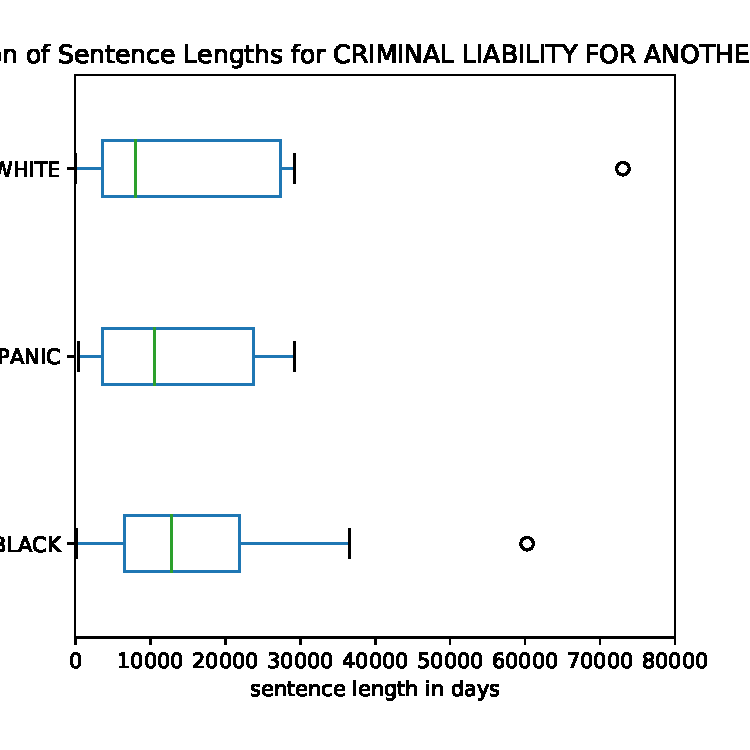
\includegraphics[scale=.6]{images/crim_lib_box.pdf}
    \caption{Distribution of sentence length of inmates convicted of criminal liability, blocked by race}
    \label{fig:my_label}
\end{figure}
    
    Again we can notice that the distributions don't seem to be all that
different. However, we can examine kurtosis to see if there is a
significant difference between these distributions that is lost in a box
plot.

    \begin{Verbatim}[commandchars=\\\{\}]
White Kurtosis for
	CRIMINAL LIABILITY FOR ANOTHER PERSON: 12.421485976410926
Black Kurtosis for
	CRIMINAL LIABILITY FOR ANOTHER PERSON: 23.752981544095174
Hispanic Kurtosis for
	CRIMINAL LIABILITY FOR ANOTHER PERSON: 0.5345890525784038

    \end{Verbatim}

    Here it is made clear that Blacks and Hispanics are much more likely to
receive an extreme sentence than other racial groups for the crime of
criminal liability.

Following is a sample of a few offenses, the distributions of sentence
lengths, and the kurtosis of those distributions.

\begin{figure}[H]
    \centering
    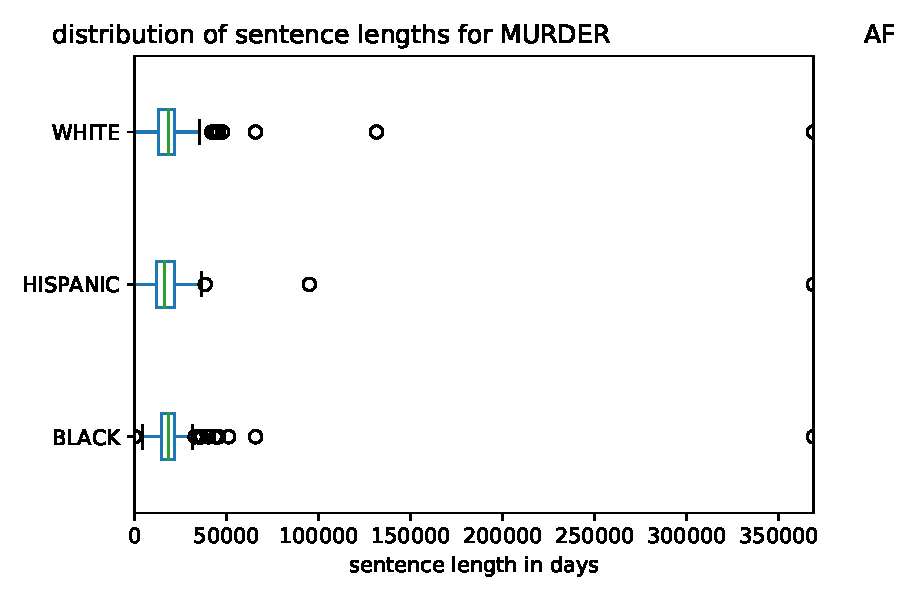
\includegraphics[scale=.6]{images/MURDEr_box.pdf}
    \caption{Distribution of sentence length of inmates convicted of murder, blocked by race}
    \label{fig:my_label}
\end{figure}
    
    \begin{Verbatim}[commandchars=\\\{\}]
White Kurtosis: 3.815929855470677
Black Kurtosis: 35.42506786574221
Hispanic Kurtosis: 23.661202825848072

    \end{Verbatim}

\begin{figure}[H]
    \centering
    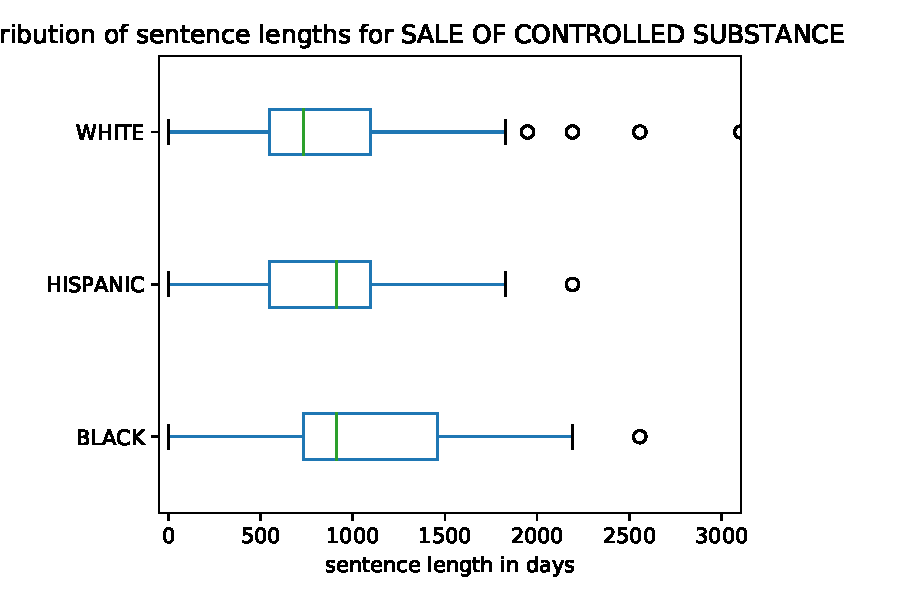
\includegraphics[scale=.6]{images/SALE OF CO_box.pdf}
    \caption{Distribution of sentence length of inmates convicted of sale of controlled substances, blocked by race}
    \label{fig:my_label}
\end{figure}
    
    \begin{Verbatim}[commandchars=\\\{\}]
White Kurtosis: 3.2523247666826185
Black Kurtosis: 4.946745832035741
Hispanic Kurtosis: 40.024525483281515

    \end{Verbatim}

\begin{figure}[H]
    \centering
    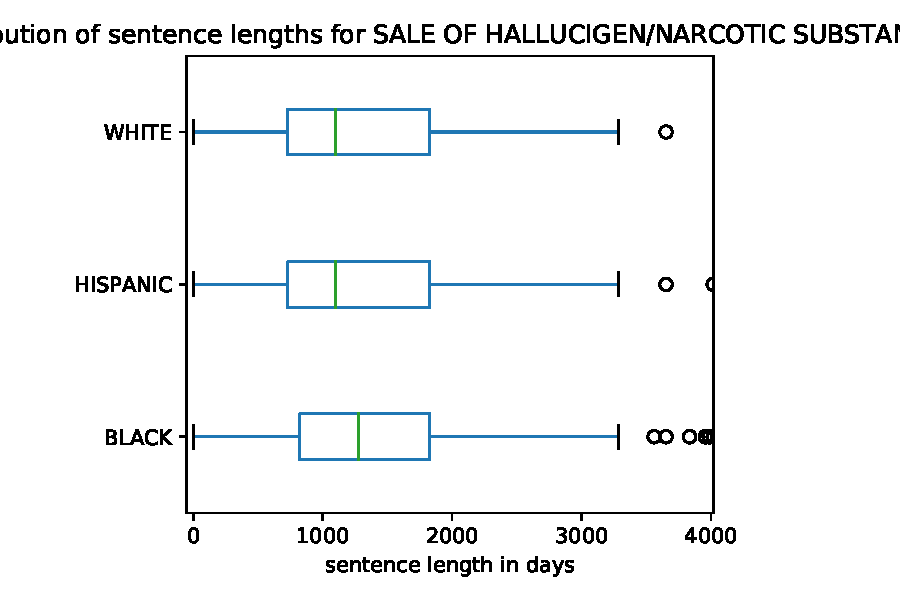
\includegraphics[scale=.6]{images/SALE OF HA_box.pdf}
    \caption{Distribution of sentence length of inmates convicted of sale of hallucinogen/narcotic substance, blocked by race}
    \label{fig:my_label}
\end{figure}
    
    \begin{Verbatim}[commandchars=\\\{\}]
White Kurtosis: 26.642120595723625
Black Kurtosis: 123.56848013313629
Hispanic Kurtosis: 0.751155900894612

    \end{Verbatim}

\begin{figure}[H]
    \centering
    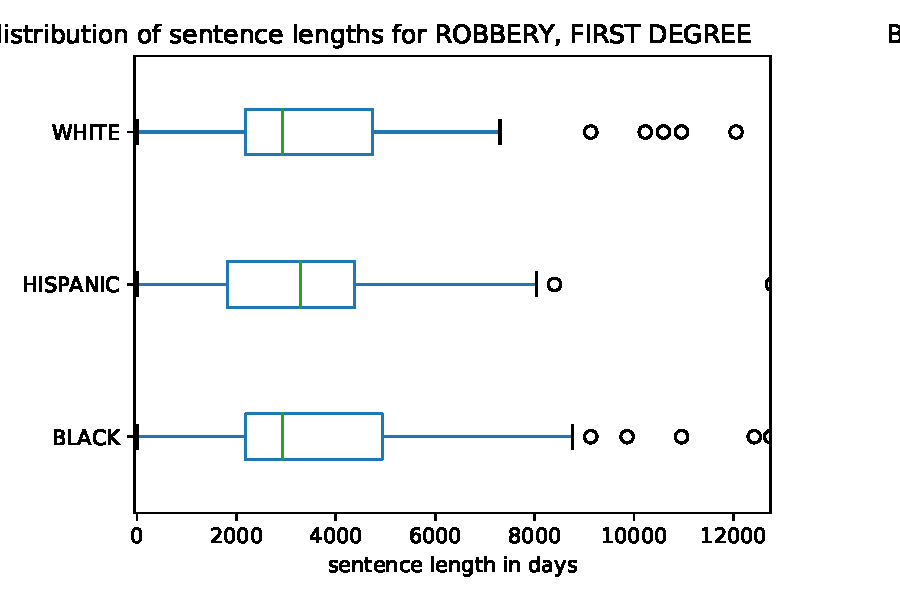
\includegraphics[scale=.6]{images/ROBBERY, F_box.pdf}
    \caption{Distribution of sentence length of inmates convicted of robbery, blocked by race}
    \label{fig:my_label}
\end{figure}
    
    \begin{Verbatim}[commandchars=\\\{\}]
White Kurtosis: 41.205491339214646
Black Kurtosis: 75.82664857484097
Hispanic Kurtosis: 99.72485672864623

    \end{Verbatim}

    Here we can see that in many cases Blacks and Hispanics are treated
differently when it comes to sentencing and incarceration.

    \hypertarget{conclusion}{%
\section{Conclusion}\label{conclusion}}

The American criminal justice system had been criticized by many. Some
claim that it is an extension of slavery, others claim that is biased
and broken, while still others claim that it is effective\cite{eji}. Dozens of
organizations study the American prison system with the goal of
reforming it, while private, for profit, prisons lobby to maintain the
status quo. We have explored a few of the ways in which the American
criminal justice system is biased, though understanding the biases is
only the first step to formulating sound policy that can affect positive
change. I hope the facts and opinions presented in this report become
impetus to research further and understand the ways in which American
society continues to disenfranchise Americans of color today.


    % Add a bibliography block to the postdoc
\pagebreak

\nocite{*}
\printbibliography
    
\end{document}
